

\tikzset{every picture/.style={line width=0.75pt}} %set default line width to 0.75pt        

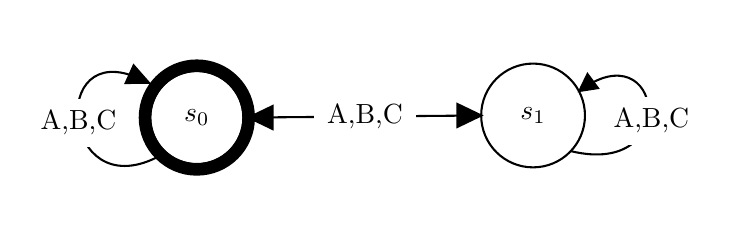
\begin{tikzpicture}[x=0.75pt,y=0.75pt,yscale=-1,xscale=1]
%uncomment if require: \path (0,300); %set diagram left start at 0, and has height of 300

%Shape: Circle [id:dp03041330611239501] 
\draw   (100,136) .. controls (100,122.19) and (111.19,111) .. (125,111) .. controls (138.81,111) and (150,122.19) .. (150,136) .. controls (150,149.81) and (138.81,161) .. (125,161) .. controls (111.19,161) and (100,149.81) .. (100,136) -- cycle ;
%Shape: Circle [id:dp06778329694496121] 
\draw   (262,135) .. controls (262,121.19) and (273.19,110) .. (287,110) .. controls (300.81,110) and (312,121.19) .. (312,135) .. controls (312,148.81) and (300.81,160) .. (287,160) .. controls (273.19,160) and (262,148.81) .. (262,135) -- cycle ;
%Straight Lines [id:da33786910107719414] 
\draw    (262,135) -- (150,136) ;


%Shape: Circle [id:dp28310457724521987] 
\draw   (102.6,136) .. controls (102.6,123.63) and (112.63,113.6) .. (125,113.6) .. controls (137.37,113.6) and (147.4,123.63) .. (147.4,136) .. controls (147.4,148.37) and (137.37,158.4) .. (125,158.4) .. controls (112.63,158.4) and (102.6,148.37) .. (102.6,136) -- cycle ;
%Shape: Circle [id:dp9488628075819832] 
\draw  [line width=4.5]  (100,136) .. controls (100,122.19) and (111.19,111) .. (125,111) .. controls (138.81,111) and (150,122.19) .. (150,136) .. controls (150,149.81) and (138.81,161) .. (125,161) .. controls (111.19,161) and (100,149.81) .. (100,136) -- cycle ;
%Curve Lines [id:da15096966683993052] 
\draw    (105.72,155.18) .. controls (59.72,178.18) and (53.3,97.2) .. (97.3,117.2) ;


%Shape: Triangle [id:dp024620734385268905] 
\draw  [fill={rgb, 255:red, 0; green, 0; blue, 0 }  ,fill opacity=1 ] (101.95,119.29) -- (90.74,119.35) -- (94.56,110.87) -- cycle ;
%Curve Lines [id:da3650058854241438] 
\draw    (309.3,123.2) .. controls (349.3,93.2) and (359.3,165.2) .. (305.3,152.2) ;


%Shape: Triangle [id:dp6528725824186807] 
\draw  [fill={rgb, 255:red, 0; green, 0; blue, 0 }  ,fill opacity=1 ] (309.3,123.2) -- (313.22,115.05) -- (318.23,121.81) -- cycle ;
%Shape: Triangle [id:dp5954374173670742] 
\draw  [fill={rgb, 255:red, 0; green, 0; blue, 0 }  ,fill opacity=1 ] (262,135) -- (250.5,140.53) -- (250.5,129.47) -- cycle ;
%Shape: Triangle [id:dp7130809704304564] 
\draw  [fill={rgb, 255:red, 0; green, 0; blue, 0 }  ,fill opacity=1 ] (150,136) -- (161.5,130.47) -- (161.5,141.53) -- cycle ;

% Text Node
\draw (125,136) node  [align=left] {$s_0$};
% Text Node
\draw (287,135) node  [align=left] {$s_1$};
% Text Node
\draw  [color={rgb, 255:red, 255; green, 255; blue, 255 }  ,draw opacity=1 ][fill={rgb, 255:red, 255; green, 255; blue, 255 }  ,fill opacity=1 ]  (182,124.5) -- (230,124.5) -- (230,146.5) -- (182,146.5) -- cycle  ;
\draw (206,135.5) node  [align=left] {A,B,C};
% Text Node
\draw  [color={rgb, 255:red, 255; green, 255; blue, 255 }  ,draw opacity=1 ][fill={rgb, 255:red, 255; green, 255; blue, 255 }  ,fill opacity=1 ]  (44,127.5) -- (92,127.5) -- (92,149.5) -- (44,149.5) -- cycle  ;
\draw (68,138.5) node  [align=left] {A,B,C};
% Text Node
\draw  [color={rgb, 255:red, 255; green, 255; blue, 255 }  ,draw opacity=1 ][fill={rgb, 255:red, 255; green, 255; blue, 255 }  ,fill opacity=1 ]  (320,126.5) -- (368,126.5) -- (368,148.5) -- (320,148.5) -- cycle  ;
\draw (344,137.5) node  [align=left] {A,B,C};


\end{tikzpicture}
